\section{Evaluation of Eye Tracking Signal Quality Requirements}

To better understand ET's role in future contextual AI systems, we first estimate the ET signal quality needed for accurate gaze-based selection of physical objects.  Contextual AI models that collaborate with users would benefit from knowledge of users' real-world interests.  ET is a promising signal to capture the user's attention, both at one point in time~\cite{konrad_gazegpt_2024}, or continuously to build historical context.  We hypothesize that the visual angle subtended by objects that users ``look at'' defines a lower bound on ET signal accuracy.  By measuring the visual angle expressed by nearby objects, we can approximate the ET accuracy required to consistently track a user's point of focus.

To investigate accuracy requirements, we analyze objects that are nearby in the user's field of view (FOV) during daily household tasks, then relate the object size statistics to ET signal quality requirements.  Because we expect humans and AI agents to collaborate in daily life, it is important for the ET system to achieve an accuracy which allows consistent, accurate attention modeling in a broad set of scenarios~\cite{feit2017toward}.  Individuals are far more likely to look at or interact with objects in the immediate vicinity~\cite{ballendat_proxemic_2010}, so we constrain this analysis to objects which are nearby candidates for interaction.

\subsection{Dataset}

For this analyses, we use a subset of the Aria Digital Twins (ADT) dataset~\cite{pan_adt_2023}.  The ADT dataset contains egocentric recordings of daily-life tasks in indoor environments.  We analyze the recordings in the furnished apartment scene where one user performs tasks (we omit multiple-user recordings to better focus on human-object interaction rather than social interactions), totaling 93 recordings and $\sim$3 hours of footage.  Designed to model real-world household scenarios, these recordings span the following tasks:  decorating, cooking, working, cleaning, and object examination.

In addition to the ET signal (median error $= 1.5\degree$) provided by Project Aria glasses~\cite{engel_aria_2023}, the ADT dataset contains ground-truth information about physical objects in the scene.  Each object's position, orientation, bounding box, and segmentation region is tracked throughout the recording, with median tracking error of $5 mm$.  This ground-truth data enables the analysis of object visual statistics at a fine scale, detection of human-object interactions, and accurate placement of gaze on objects.  There are 396 distinct household objects tracked in the dataset, with varying presence across the different tasks and recordings.

\subsection{Object Visual Size in Relation to Eye Tracking Error}

ET spatial error is the measured bias between the ground truth and estimated gaze positions.  This error persists following techniques such as ET calibration and fixation detection~\cite{schuetz_eye_2022}.  We measure spatial error as an angular offset between the user's true gaze point and computed value.  We wish to approximate the influence of ET spatial error in placing fixations on objects, to better inform how reliably an ET system could convey a user's attention on world objects.

Our metrics to predict ET accuracy needs are derived from object visual size --- the visual angle spanned by the object relative to the user's FOV.  Visual size is related to both the physical size of an object and its distance from the user.  We model object visual size from the total segmentation area $A_{{}_{seg}}$ of an object in a linear camera model, which measures degrees$^2$ occupied by the object.  To convey visual size against a one-dimensional ET error requirement $err_{{}_{ET}}$, we convert visual size to the approximate \textbf{radius} of the object. $err_{{}_{ET}} \ \leq \ \sqrt{A_{{}_{seg}} / \pi}$.  This inequality approximates an \textbf{average case} for the ET error requirement, and is valid when objects have roughly uniform dimensions.  To account for non-uniform objects, we compute a more \textbf{conservative} ET error as $1 / 2$ the \textbf{minor axis} span $L_{min}$ of the object's segmentation region: $err_{{}_{ET}\ low} \ \leq \ 1 / 2 \ L_{min}$.  \autoref{fig:et_relationship} illustrates these metrics and the relationship between ET error requirements and object visual size.

\begin{figure}[t]
 \centering
 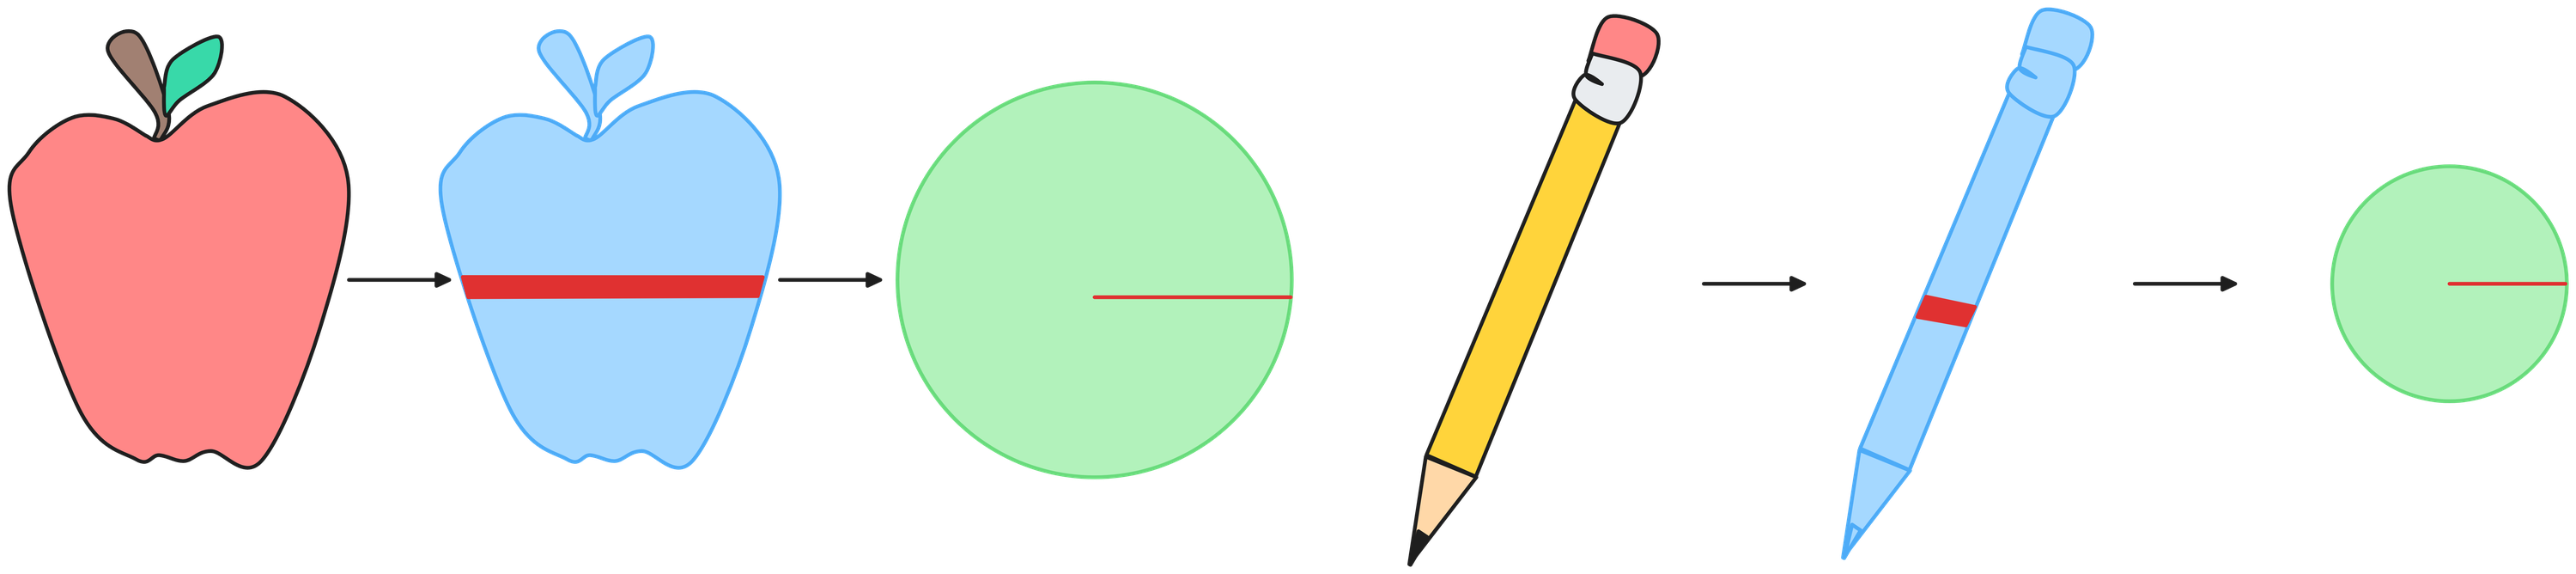
\includegraphics[width=\linewidth]{figures/segment_illustration_flat.png}
 \caption{Illustration of eye tracking spatial error and object visual size measurements.  As an average case measurement, object segmentation area can be mapped to a circular region, with the radius reflecting the eye tracking accuracy requirement (\textcolor{red}{thin bars}).  Alternatively, $1 / 2$ minor axis span $L_{min}$ (\textcolor{red}{thick bars}) is a stricter bound for measuring non-uniform objects.}
 \label{fig:et_relationship}
\end{figure}

\subsection{Protocol}

We approximate the ET requirements for daily use by observing the household tasks being performed in the ADT dataset~\cite{pan_adt_2023}.  We measure the distributions of object visual sizes for $err_{{}_{ET}}$ and $err_{{}_{ET}\ low}$.  To better inform various contextual AI applications, we specify the ET requirements across different interaction spaces, namely:
\begin{enumerate}  [topsep=0pt]
    \item \textbf{Near-field objects:} all objects within 1 meter of the participants.
    \item \textbf{Mid-field objects:} all objects between 1 - 2 meters of the participants.
    \item \textbf{Interacted objects:} all objects being physically interacted with (held, pressed, pushed, etc.) by the participants, with a start / stop padding of 1 second for the interaction.
    \item \textbf{Fixated objects:} all objects within 2 meters fixated on by participants' gaze as they navigate the scenes.
\end{enumerate}

\begin{figure*}[t]
    \centering
    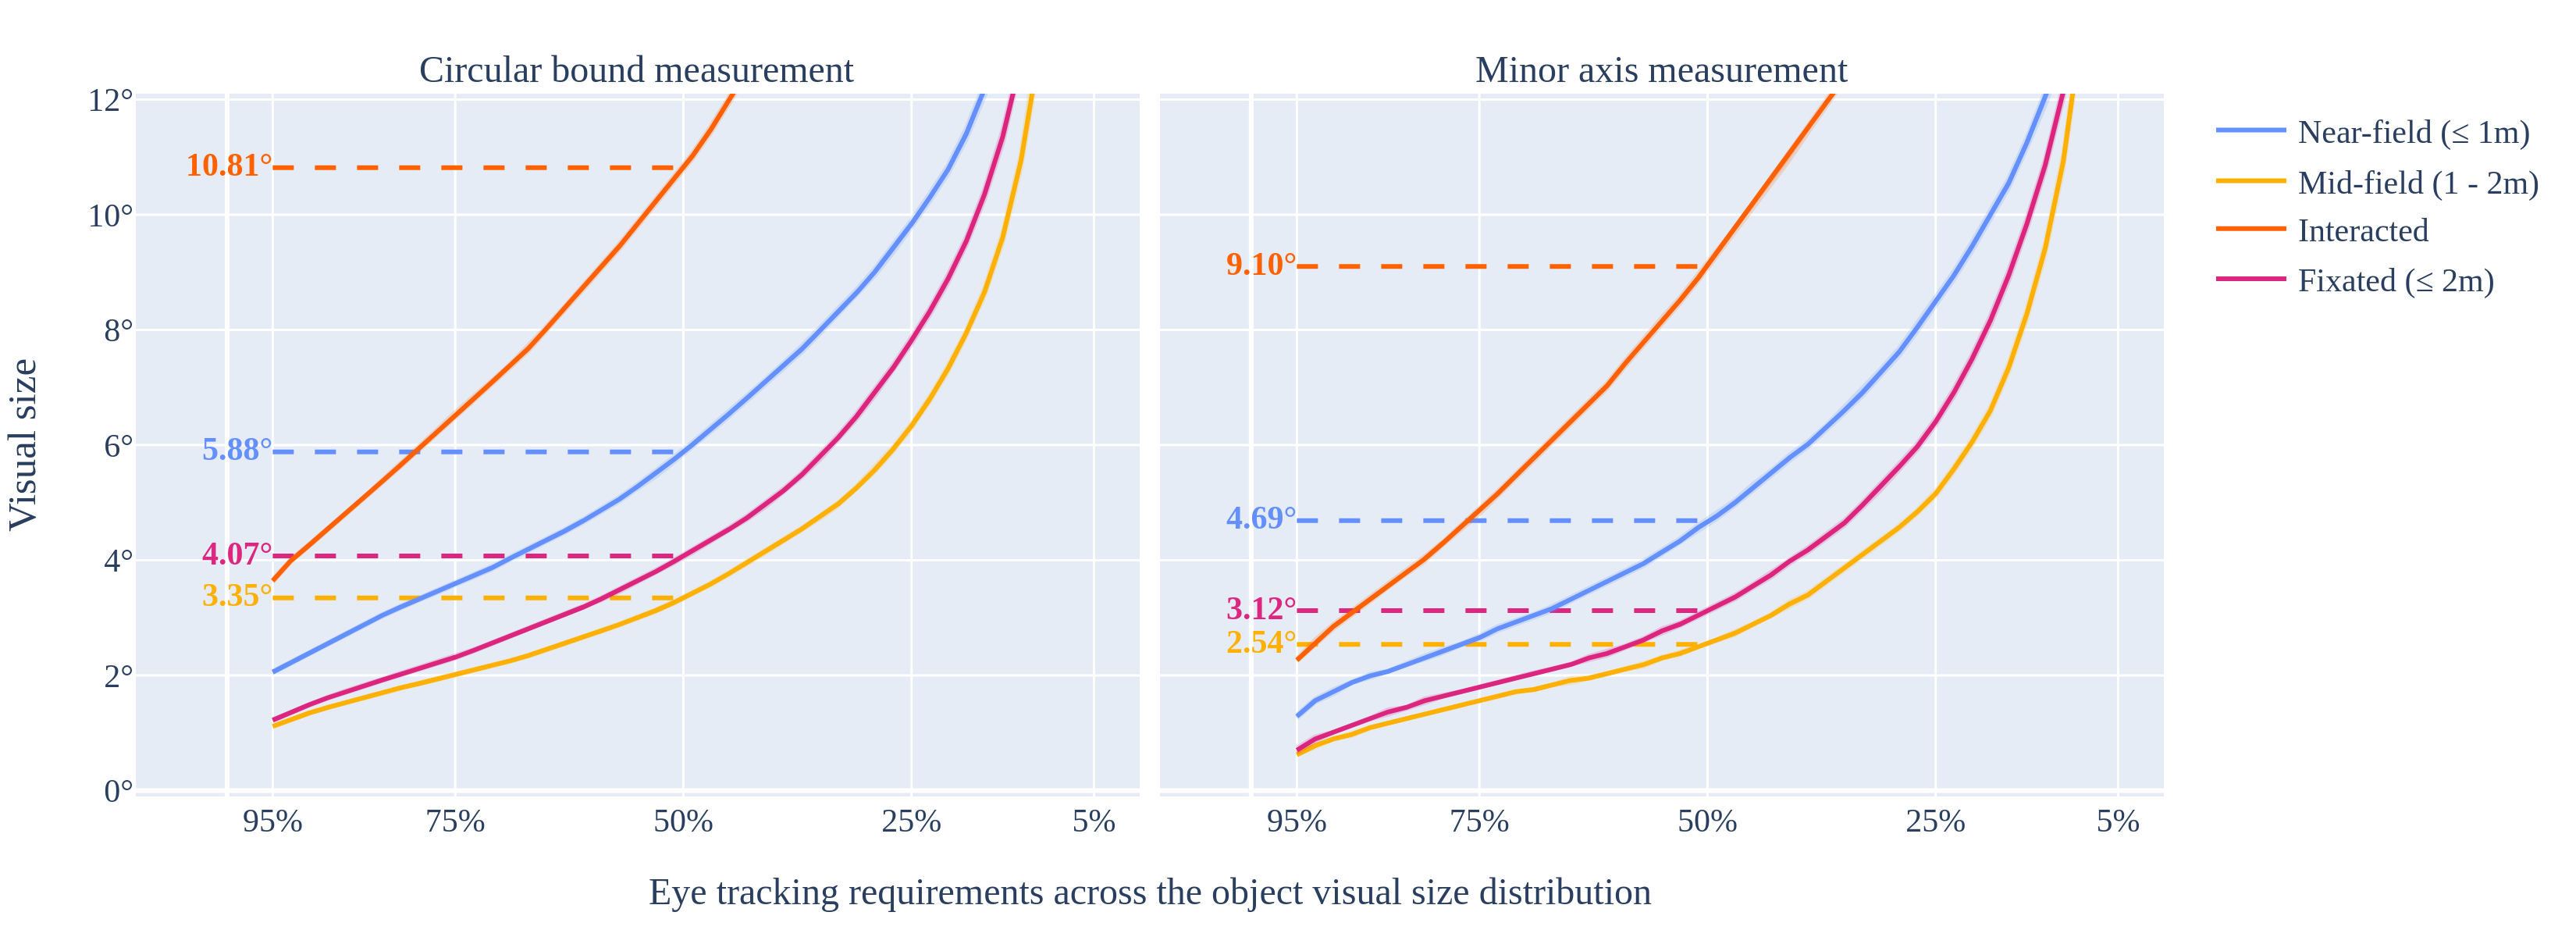
\includegraphics[width=\linewidth]{figures/vis_size.png}
    \caption{Eye tracking accuracy requirements to place gaze accurately within in the ADT dataset, where users performed household actions in an indoor environment~\cite{pan_adt_2023}  Near-field and mid-field measurements consider all objects present in the user's field of view.  Interacted objects are being actively manipulated by the user, and fixated objects consider those being directly gazed at.}
    \label{fig:visual_sizes}
\end{figure*}

\subsection{Results}
\label{sec:accuracy_results}

The \textbf{interacted} measurement aggregates object statistics when being manually interacted with, including picking up, pushing, pressing, etc. The \textbf{near-field} ($\leq$ 1 meter) and \textbf{mid-field} (1 - 2 meters) measurements reflect the visual FOV occupied by \textit{every} object in the environment within the distance threshold.  \textbf{Fixation} measurements consider objects that are within 2 meters of the participant at the time of fixation.  Considering ADT's household scenarios, the \textbf{interacted} and \textbf{fixation} categories reflect the distribution of objects likely to be of interest during daily tasks.

To estimate ET accuracy requirements, we compute the entire distribution of object visual sizes recorded in camera projection space. To place gaze on an object of average (projected) size 50\% of the time, we measure at the distribution's 50\% mark.  These measurements can help to inform system design; while 50\% reliability may be \textit{useful supporting context} in a broader contextual AI agent, a system relying heavily on ET may aim for higher coverage.  The distributions for each interaction scenario are seen in \autoref{fig:visual_sizes}.

%Recall that angular \textbf{radius} is used to represent the \textbf{average case} ET requirements, and \textbf{minor axis} span as a more \textbf{conservative} measurement.  
Wearable ET accuracy is known to suffer in dynamic conditions~\cite{onkhar_tobii_2023}, yet recent devices remain quite accurate in unconstrained settings\footnote{\url{https://www.tobii.com/products/eye-trackers/wearables/tobii-pro-glasses-3}}\footnote{\url{https://pupil-labs.com/products/neon}}.  Assuming a device with $\leq 3 \degree$ accuracy during daily wear, our results indicate that the majority of fixated objects (radius average=$4.07\degree$; minor axis=$3.12\degree$), the majority of objects in the near-field (radius=$5.88\degree$; minor axis=$4.69\degree$), and nearly all interacted objects (radius=$10.81\degree$; minor axis=$9.10\degree$) are reliable for placing gaze on the correct object.  Conversely, objects in the mid-field (radius=$3.3\degree$; minor axis=$2.54\degree$) will be somewhat unreliable at this signal quality, where roughly half of objects are not able to be detected.